\chapter{Installing Nova}
\lettrine[lines=3]{W}{} ith the basics and theory behind us, it is time to get hands-on with Nova and install the code on a server. 
In this chapter, we will walk through the installation and configuration of Nova on a single node with CentOS 6.2 packages.
\section{Single Node Install}
 \paragraph{} CentOS 6.2 is available for i386 and x86\_64, as a DVD-assembly (4.6 Gb),
 the image of minimum installation (285 MB) and the reduced image for network installation - netinstall.iso (162 MB).
For our project end of year we used 
CentOS-6.2-i386-bin-DVD.\par

\newpage
\subsection{Installing CentOS:}
 
\begin{figure}[!h]
\center
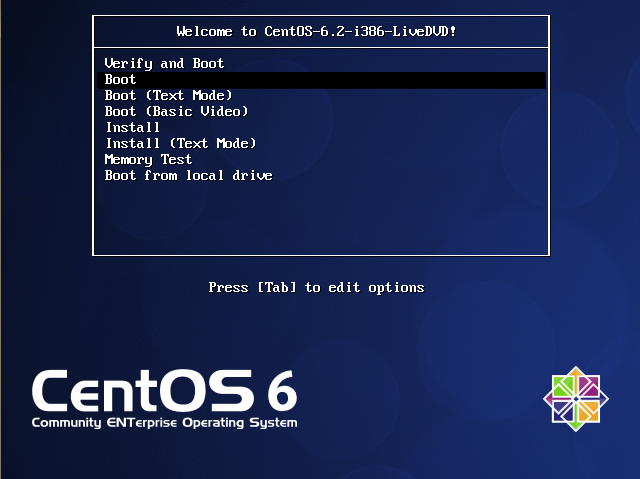
\includegraphics[width=13cm, height=8cm]{./images/install/accueil}
\caption{Installing CentOS 6.2- Home screen }
\end{figure}

\begin{figure}[!h]
 \center
 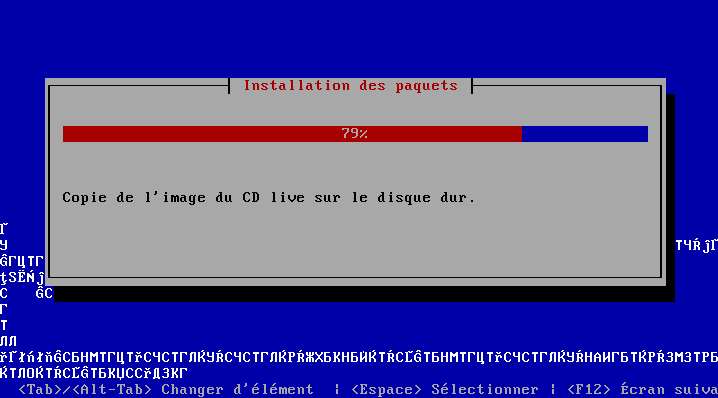
\includegraphics[width=13cm, height=8cm]{./images/install/install}
 \caption{Installing CentOs 6.2- installing packages}
\end{figure}

\newpage

\begin{figure}[!h]
 \center
 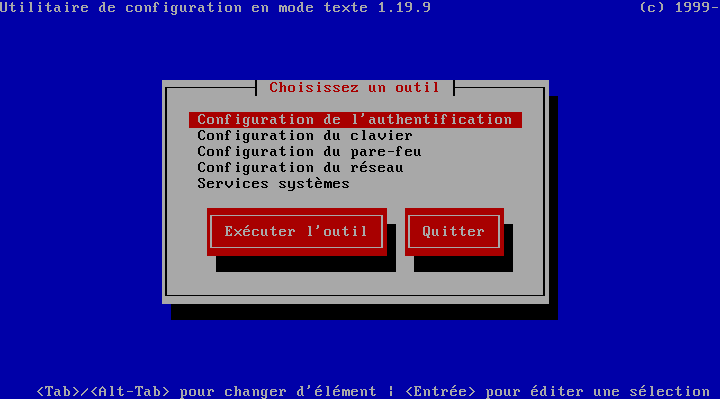
\includegraphics[width=13cm, height=9cm]{./images/install/conf}
 \caption{Installing CentOs 6.2- configuration}
\end{figure}

\begin{figure}[!h]
 \center
 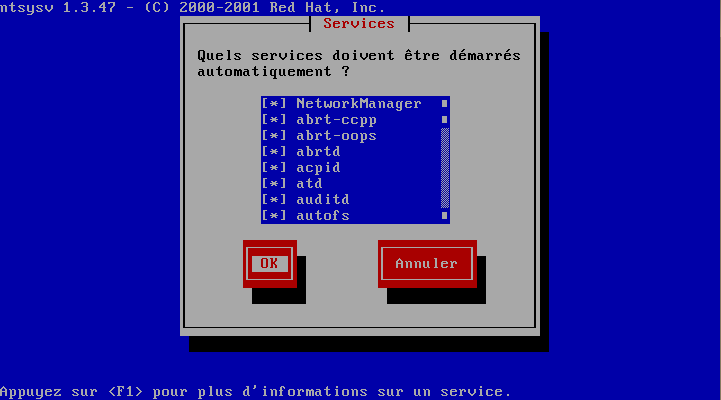
\includegraphics[width=13cm, height=9cm]{./images/install/service}
 \caption{Installing CentOs 6.2- service configuration}
\end{figure}



\newpage
\subsection{Include Repositories:}
\paragraph{}For CentOS 6.2 we need only DVD installation or an Internet connection. All dependencies included in our repository. To include our repository we create a file gd-openstack.
repo in \textbf{/etc/yum.repos.d} directory with content:


\begin{lstlisting}[language={[Latex]TeX}, numbers=left, frame=single]
[gd]
name=Packages from GridDynamics
baseurl=http://yum.griddynamics.net/yum/diablo-centos
enabled=1
gpgcheck=0
priority=1

\end{lstlisting}

And addiditionaly include EPEL and CR repositories.
\begin{lstlisting}[language={[Latex]TeX},basicstyle=\small, frame=single]
# yum install centos-release-cr
# rpm -Uvh http://download.fedora.redhat.com/pub/epel
/6/x86_64/epel-release-6-5.noarch.rpm
\end{lstlisting}

\subsection{Install nova from packages:}
\paragraph{Cloud Controller:}
We Install MySQL as oour database with the mysql-server package.\par

\begin{lstlisting}[language={[Latex]TeX}, frame=single]
# yum install mysql mysql-server
# yum install openstack-nova-node-full
# yum install euca2ools
# yum install python-novaclient
# yum install MySQL-python

\end{lstlisting}

\paragraph{}All other packages will be installed as dependencies automatically.

\subsection{Create MySQL database on Cloud Controller:}
\paragraph{}Nova uses MySQL to store information about running VMs (PostgreSQL is also possible to use).


\begin{lstlisting}[language={[Latex]TeX}, frame=single]
# mysqladmin -uroot -p -f drop nova
# mysqladmin -uroot -p create nova
\end{lstlisting}
With the database created, we now need to make an account for the user nova. We’ll just use some quick SQL statements to grant privileges 
and set the password before we login to make sure we did it correctly.We used this script (we run it without arguments) to prepare our database for nova:

\begin{lstlisting}[language={[Latex]TeX}, numbers=left, frame=single]
#!/bin/bash

DB_NAME=nova
DB_USER=nova
DB_PASS=nova
PWD=nova

HOSTS="$@"

for h in $HOSTS localhost; do
        echo "GRANT ALL PRIVILEGES ON $DB_NAME.* TO 
'$DB_USER'@'$h'IDENTIFIED BY '$DB_PASS';" | mysql -uroot -p
$PWD mysql
done
echo "GRANT ALL PRIVILEGES ON $DB_NAME.* TO $DB_USER IDENTIFIED 
BY '$DB_PASS';" | mysql -uroot -p$PWD mysql
echo "GRANT ALL PRIVILEGES ON $DB_NAME.* TO root IDENTIFIED BY
'$DB_PASS';" | mysql -uroot -p$PWD mysql

nova-manage db sync

\end{lstlisting}
\paragraph{}The nova-manage db command is rarely used except for troubleshooting and upgrades. It has two subcommands: sync and version. 
The sync subcommand will upgrade the database scheme for new versions of Nova and the version will report the current version.\par

\paragraph{}To upgrade scheme versions, use the nova-manage db sync(the last of our script). 
This should be rarely used unless we are installing from source(in our case) or upgrading our installation. 
If there are pending scheme migrations, it will apply those to your database. If there are not, it will return nothing.\par
\paragraph{}To view the database scheme version, we use the db version arguments:\par

\begin{lstlisting}[language={[Latex]TeX}, frame=single]
# nova-manage db version
\end{lstlisting}

\newpage

\subsection{Run services:}
\begin{lstlisting}[language={[Latex]TeX}, frame=single]
# service rabbitmq-server start
# service libvirtd start
# service nova-api start
# service nova-direct-api start
# service nova-compute start
# service nova-network start
# service nova-objectstore start
# service nova-scheduler start
# service glance-api start
# service glance-registry start
\end{lstlisting}
\paragraph{}Services can be monitored through the nova-manage command on a service or host basis. 
With the service, you can either view or actively manage services. For example, you can query a host for the services that it currently offers,
 or simply list all the services that are available. This is an essential command for testing or troubleshooting your deployment. 
Below is an example that walks through the full array of of service subcommands:
 listing services, enabling and disabling services, and describing resources on a host.\par



\begin{lstlisting}[language={[Latex]TeX}, frame=single]
# nova-manage service list nova-controller nova-compute
# nova-manage service disable nova-controller nova-scheduler
# nova-manage service list
# nova-manage service enable nova-controller nova-scheduler
# nova-manage service list
# nova-manage service describe_resource nova-controller

\end{lstlisting}

\paragraph{}nova-manage service also allows we to update resources that are available on a particular host. This is only applies to compute hosts.

\subsection{Configuration:}
\paragraph{}Nova administration is accomplished through a tool called nova-manage. 
Most commands take the form nova-manage command subcommand and any necessary arguments. At any time, 
you can see help for nova-manage by leaving off any arguments, subcommands, or commands.\par

\textbf{Create the network configuration:}

\begin{lstlisting}[language={[Latex]TeX}, frame=single]
# nova-manage network create novanetwork 10.0.0.0/8 1 64
\end{lstlisting}
\paragraph{}we choose fixed (private) IP address range. 
we use 10.0.0.0/8 range as long as this does not conflict with our current network settings. 
\paragraph{}For this command, the IP address is the cidr(Classless Inter-Domain Routing) notation for our netmask,
The value 1 is the total number of networks we made, and the 64 value is the number of IP addresses in each network. 

\paragraph{}Nova has a trio of nova-manage networking commands: network, fixed, and floating. The nova-manage network is the most powerful. 
It allows you to list, create, and delete networks within the Nova database.For example:\par
\paragraph{}We used this command for listing:\par

\begin{lstlisting}[language={[Latex]TeX}, frame=single]
# nova-manage network list
\end{lstlisting}

\paragraph{}The fixed command simply allows we to view the fixed IP address mappings to hostname, host, and MAC address.
esults of the command (it goes on to show the every IP address in the mapping):

\begin{lstlisting}[language={[Latex]TeX}, frame=single]
# nova-manage fixed list
\end{lstlisting}

\paragraph{}The floating command is very similar to the fixed command except that it manipulates public IP addresses.\par
%%%%%%%%%%%%%%%%%%%%%%%%%%%%%%%%%%%%%%%%%%%%%%%%%%%%Nova Administrator %%%%%%%%%%%%%%%%%%%%%%%%%%%%%%%%%%%%%%%%%%%%%%%%%%%%%%%%%%%%%%%%%%%%%%%%%%%%%%%%%%%%
\textbf{Creating User and Projects}

\paragraph{} The first step is using our new Nova installation is to create a user. 
This is a multi-step process that uses the nova-manage utility to create a project.\par
\textbf{Create a Nova administrator:}

\begin{lstlisting}[language={[Latex]TeX}, frame=single]
# nova-manage user admin nova
\end{lstlisting}
\newpage
\textbf{After that we can see an access key and a secret key export:}
\begin{lstlisting}[language={[Latex]TeX}, frame=single]
export EC2_ACCESS_KEY=e4764179-fecd-49e5-8f62-70418ffb94bb
export EC2_SECRET_KEY=9329a8c3-ad93-4176-b350-0099a43527ab
\end{lstlisting}

\textbf{Create a project for the user we created:}

\begin{lstlisting}[language={[Latex]TeX}, frame=single]
# nova-manage project create IRT nova
\end{lstlisting}

\textbf{Download credentials for ower user/project}

\begin{lstlisting}[language={[Latex]TeX}, frame=single]
# nova-manage project zipfile IRT nova
\end{lstlisting}

\textbf{Unzip and source credentials:}

\paragraph{} The final step will produce a zip-compressed file called nova.zip. Now we uncompress the credential zip file and source the resulting novarc  in ower current working directory. 
This will set a number of environmental variables needed to access your Nova installation with other utilities. 
If we are creating this user on behalf of another user, we will need to give him this zipfile.\par
\textbf{ We unzip it with this command:}
\begin{lstlisting}[language={[Latex]TeX}, frame=single]
# unzip nova.zip
\end{lstlisting}
\paragraph{}We see these files extract:\par 
\begin{lstlisting}[language={[Latex]TeX}, frame=single]
Archive:  nova.zip
 extracting: novarc
 extracting: pk.pem
 extracting: cert.pem
 extracting: nova-vpn.conf
 extracting: cacert.pem
\end{lstlisting}

%%%%%%%%%%%%%%%%%%%%%%%%%%%%%%%%%%%%%%%%%%%%%%%%%%%%%%%%%%%%%%%%%%%%%%%Register an image%%%%%%%%%%%%%%%%%%%%%%%%%%%%%%%%%%%%%%%%%%%%%%%%%%%%%%%%%%%%%%%%%%%%%
\newpage
\subsection{Register an image:}
\paragraph{}Instances are created from registered images. Before we can launch instances, we need to upload a virtual disk image into Nova. 
There are a number of different images that you can use with your Nova installation. 
You can also make your own images.\par
\textbf{Get a working image with kernal and initrd:}
\begin{lstlisting}[language={[Latex]TeX}, frame=single]
# wget http://smoser.brickies.net/ubuntu/ttylinux-uec
/ttylinux-uec-amd64-12.1_2.6.35-22_1.tar.gz
\end{lstlisting}
\begin{lstlisting}[language={[Latex]TeX}, frame=single]
# tar -xvf ttylinux-uec-amd64-12.1_2.6.35-22_1.tar.gz
\end{lstlisting}



\textbf{Bundle, upload, and register the kernel, initrd, and image}
\newline
\textbf{Kernel:}
\begin{lstlisting}[language={[Latex]TeX}, frame=single]
# euca-bundle-image -i ttylinux-uec-amd64-12.1_2.6.35-22_1-vmlinuz 
--kernel true
# euca-upload-bundle -b kernel-bucket -m /tmp
/ttylinux-uec-amd64-12.1_2.6.35-22_1-vmlinuz.manifest.xml
# euca-register kernel-bucket
/ttylinux-uec-amd64-12.1_2.6.35-22_1-vmlinuz.manifest.xml
\end{lstlisting}
\textbf{Initrd:}
\begin{lstlisting}[language={[Latex]TeX}, frame=single]
\begin{lstlisting}[language={[Latex]TeX}, frame=single]
# euca-bundle-image -i ttylinux-uec-amd64-12.1_2.6.35-22_1-initrd 
--ramdisk true
# euca-upload-bundle -b ramdisk-bucket -m /tmp
/ttylinux-uec-amd64-12.1_2.6.35-22_1-initrd.manifest.xml
# euca-register ramdisk-bucket
/ttylinux-uec-amd64-12.1_2.6.35-22_1-initrd.manifest.xml
\end{lstlisting}

\newpage

\textbf{Image:}
\begin{lstlisting}[language={[Latex]TeX}, frame=single]
# euca-bundle-image -i ttylinux-uec-amd64-12.1_2.6.35-22_1.img 
--kernel <aki name> --ramdisk <ari name>
# euca-upload-bundle -b image-bucket -m /tmp
/ttylinux-uec-amd64-12.1_2.6.35-22_1.img.manifest.xml
# euca-register image-bucket
/ttylinux-uec-amd64-12.1_2.6.35-22_1.img.manifest.xml
\end{lstlisting}

\textbf{Add a key :}

\begin{lstlisting}[language={[Latex]TeX}, frame=single]
# euca-add-keypair mykey > mykey.pem
\end{lstlisting}

\textbf{Run the vm }

\begin{lstlisting}[language={[Latex]TeX}, frame=single]
# euca-run-instances -k mykey ami-00000003
\end{lstlisting}

\paragraph{}Our instance has been launched and it is currently in the 'scheduling' state. 
If we wait a few minutes and everything goes well, it should progress to the 'running' state.
 We can check on its progress through the EC2 API with the euca-describe-instances command:

\begin{lstlisting}[language={[Latex]TeX}, frame=single]
# euca-describe-instances
\end{lstlisting}

\paragraph{}We can also use the nova utility to make the same query through the OpenStack API. With this tool, you are looking for the 'ACTIVE' status:\par

\begin{lstlisting}[language={[Latex]TeX}, frame=single]
# nova list
\end{lstlisting}
%%%%%%%%%%%%%%%%%%%%%%%%%%%%%%%%%%%%%%%%%%%%%%%%%%%%%%%%%%%%%%%%%%%%%%%%%%%%%%%%%%%%%%%%%%%%%%%%%%%%%%%%%%%%%%%%%%%%%%%%%%%%%%%%%%%%%%%%%%%%%%%%%%%%%%%%%
\section{Conclusion: }
in this chapter, we presented the step of installing nova and some commande how to manipulate them.